% ======================================================================
% Computers & Security (Elsevier) submission build.
% Compile on Overleaf with the built-in elsarticle class (no local .cls needed).
% Highlights are in highlights.txt (Elsevier wants them as a separate file).
% AUTHOR TODO before submission: see SUBMISSION_CHECKLIST.md. The empirical
% numbers below are CORRECT but currently from the single-seed (seed 42) run;
% the 5-seed mean+/-s.d. and CIs are produced by the implementation prompt in
% Q1_Refresh_2026-06/CLAUDE_CODE_IMPLEMENTATION_PROMPT.md. Spots that must be
% reconciled with that run are flagged inline with "% TODO(5-seed)".
% ======================================================================
\documentclass[review,3p,times]{elsarticle}
\usepackage{amsmath,amssymb}
\usepackage{amsthm}
\usepackage{booktabs}
\usepackage{graphicx}
\usepackage{xcolor}
\usepackage{url}
\usepackage[hidelinks]{hyperref}
\graphicspath{{figures/}}
\journal{Computers \& Security}
\newtheorem{theorem}{Theorem}
\newtheorem{definition}{Definition}
\newtheorem{corollary}{Corollary}

\begin{document}

\begin{frontmatter}

\title{Certified Canonicalization: A Detector-Agnostic Defense against
Prompt-Injection Obfuscation}

\author[ku]{Shaikhah Alkhadhr\corref{cor}}
\ead{s.alkhadhr@ku.edu.kw}
\author[ku]{Heba Alturki}
\author[ku]{Aseel Alghemlas}
\cortext[cor]{Corresponding author.}
\affiliation[ku]{organization={Information Science Department, Kuwait University},
                 country={Kuwait}}

\begin{abstract}
Prompt-injection detectors deployed in front of large language model (LLM)
pipelines are routinely evaded by orthographic and encoding obfuscation: Unicode
confusables, zero-width and Tag-block characters, and nested encodings collapse a
detector's operational recall at strict low false-positive-rate (FPR) operating
points. Existing defenses are empirical and, as recent work shows, fail once the
attacker adapts. We take a different route and prove a guarantee. We define a
deterministic, idempotent canonicalization primitive and show a decision-invariance
theorem: for any detector composed after canonicalization, the attack success rate
over the entire Unicode TR39 confusable, invisible-character, and depth-bounded
encoding closure of an input is exactly zero, with no retraining. We make the
guarantee operational by folding against the full TR39 table under a mixed-script
gate, and prove and measure that this is false-positive-neutral on genuine
non-Latin text. We then stress the primitive with a defense-aware optimizer under a
leave-one-family-out protocol: a hardened canonicalizer recovers the operational
recall of heterogeneous detectors on attack families it was not tuned on, where
base canonicalization fails. Empirically, idempotence and per-detector decision
invariance hold at 1.0 across four heterogeneous detectors, closure-soundness
reaches 1.0 under the full table (from 0.33 under a 40-entry base map), and benign
decisions are unchanged (0 flips)
on Russian, Greek, Arabic, and Chinese text. We additionally study a learned
cross-lingual invariance head and report, transparently, that it recovers
cross-lingual recall only on a monolingual encoder and is redundant once the
encoder is multilingual, with no in-domain advantage on a saturated benchmark. We
release the primitive, the certificate checker, and a reproducibility notebook.
\end{abstract}

\begin{keyword}
prompt injection \sep certified robustness \sep canonicalization \sep
Unicode confusables \sep adaptive adversarial evaluation \sep LLM security
\end{keyword}

\end{frontmatter}


% ======================================================================
\section{Introduction}
\label{sec:intro}
Large language models are increasingly deployed as the decision core of
applications that ingest untrusted text through retrieval, tool use, and
multi-party messaging. In these settings a prompt-injection attack embeds adversarial
instructions in that untrusted text to override the system's intent, exfiltrate
hidden context, or trigger unsafe actions~\cite{greshake2023,owasp2025,liu2024usenix}.
A common and cheap evasion is orthographic: the attacker disguises the malicious
text with Unicode look-alike characters (homoglyphs), zero-width and Tag-block
characters, full-width forms, or nested base64/hex/URL/ROT13
encodings~\cite{boucher2022,owasp2025}. Such perturbations leave a competent human
reader's interpretation unchanged but move the input off the distribution the
downstream detector was trained on, so its score collapses.

This collapse is most damaging precisely where deployment lives: at a strict, low
false-positive-rate (FPR) operating point. A detector that ranks well in aggregate
(high AUROC) can still lose almost all of its operational recall at a fixed
1\% FPR threshold once its score distribution is shifted by obfuscation. Two further
facts make the problem urgent. First, recent studies show that essentially every
published prompt-injection and jailbreak defense is broken once the attacker is
allowed to adapt to it: adaptive evaluations report attack success rates above
50--90\% against defenses that looked strong under static
tests~\cite{zhan2025,attacker2025,andriushchenko2024}. Second, the field has very
few defenses with any formal guarantee; certified results exist only for bounded
token edits~\cite{kumar2023} or require expressing the agent task as a
program~\cite{camel2025,melon2025}, and none cover the large, practically dominant
class of orthographic and encoding obfuscation.

We argue that prompt-injection detectors should \emph{canonicalize before they
classify}, and that, unlike a learned defense, a deterministic canonicalizer admits
a \emph{certificate}. Canonicalization maps many surface forms to a single normal
form; if that map is deterministic and idempotent, the decision of any detector
placed after it is provably constant over the entire set of inputs that share a
normal form. We turn this observation into a theorem, make it operational against
the full Unicode standard while preserving benign behavior, and validate it under
an adaptive adversary. We position the contribution as a defense \emph{primitive}
for the field rather than a property of one detector, and instantiate it in a
reference detector, CANOPI, through which we quantify residual learned behavior.

\subsection{Contributions}
\label{sec:contrib}
This paper makes four contributions.
\begin{enumerate}
\item \textbf{A decision-invariance certificate for orthographic obfuscation.} We
define the canonical closure of an input and prove (Theorem~\ref{thm:invariance})
that any detector composed after canonicalization has exactly zero attack success
over that closure, detector-agnostically and without retraining. We make the proof
obligations executable and confirm them: idempotence and per-detector decision
invariance hold at $1.0$ across four heterogeneous detectors, and closure-soundness
reaches $1.0$ under the full Unicode TR39 table (from $0.33$ under the 40-entry base map).
\item \textbf{An FPR-safe full-table fold.} Folding against the complete TR39
confusable table risks over-normalizing genuine non-Latin text. We introduce a
mixed-script gate that folds only in attack contexts and prove it cannot change
benign decisions on single-script text; empirically it produces $0$ benign decision
flips on Russian, Greek, Arabic, and Chinese inputs.
\item \textbf{Adaptive, held-out evaluation.} We stress the primitive with a
defense-aware optimizer under a leave-one-family-out protocol. A hardened
canonicalizer restores the operational recall of detectors on attack families it
was not tuned on (for example, restoring InjecGuard from $0.00$ to $0.42$ at
$1\%$ FPR), where base canonicalization fails.
\item \textbf{A transparent account of learned residual behavior.} We instantiate a
learned cross-lingual invariance head and report, against its own ablations, that
it offers no in-domain advantage on a saturated benchmark and recovers cross-lingual
recall only when the backbone encoder is monolingual, becoming redundant once the
encoder is multilingual. We report this negative-leaning result in full.
\end{enumerate}
All artifacts (the canonicalization package, the certificate checker, the
defense-aware attacker, and a one-run reproducibility notebook) are released.

\subsection{Paper organization}
Section~\ref{sec:related} reviews obfuscation attacks, detectors, canonicalization,
adaptive evaluation, and certified defenses. Section~\ref{sec:threat} states the
threat model and scope. Section~\ref{sec:method} defines the canonicalization
primitive, the certificate, the FPR-safe fold, and the reference detector.
Section~\ref{sec:setup} describes the datasets, detectors, metrics, protocol, and
research questions. Section~\ref{sec:results} reports results.
Section~\ref{sec:discussion} discusses implications and limitations, and
Section~\ref{sec:conclusion} concludes.

% ======================================================================
\section{Background and related work}
\label{sec:related}

\subsection{Prompt injection and orthographic obfuscation}
Prompt injection exploits the inability of an LLM pipeline to separate trusted
instructions from untrusted data~\cite{greshake2023,liu2024usenix,owasp2025}.
Direct injection arrives through the user channel; indirect injection is smuggled
through retrieved documents, tool outputs, or third-party content. Orthographic and
encoding obfuscation is a cross-cutting evasion: homoglyph substitution and
invisible characters~\cite{boucher2022}, full-width and compatibility variants,
and nested encodings all preserve human-readable intent while defeating
surface-form detectors. The same channel is exploited by encoding and
low-resource-language jailbreaks, which places part of the jailbreak surface within
the scope of an input-normalization defense.

\subsection{Detectors and guardrails}
Deployed defenses include fine-tuned classifiers such as
InjecGuard/PIGuard with its NotInject over-defense benchmark~\cite{li2025injecguard},
PromptShield tuned for the low-FPR regime~\cite{promptshield2025}, the
game-theoretic DataSentinel detector~\cite{datasentinel2025}, and production guard
models~\cite{inan2023llamaguard}. Architectural defenses move the trust boundary into
the model through instruction-hierarchy training~\cite{wallace2024}, structured
queries~\cite{struq2025}, and preference optimization~\cite{secalign2025}. A
recurring weakness, which our evaluation foregrounds, is that detectors report
aggregate ranking metrics and rarely a fixed low-FPR operating point or its benign
cost.

\subsection{Canonicalization and the Unicode standard}
The Unicode Consortium's Technical Standard 39 (UTS\#39) defines the confusables
mapping that underlies principled homoglyph folding~\cite{uts39}, and the OWASP
LLM Top-10 explicitly recommends canonicalization as a pre-classification step for
prompt injection~\cite{owasp2025}. Canonicalization as a defense is therefore not
itself new. Our contribution is to give it a certificate, to make the fold safe
against the full standard, and to evaluate it adaptively, none of which prior
treatments provide.

\subsection{Adaptive evaluation}
The decisive recent finding is that defenses which look strong under static attacks
collapse under a defense-aware optimizer. Independent 2025 studies break eight and
twelve published defenses respectively, with attack success above 50\% and
90\%~\cite{zhan2025,attacker2025}, and per-model adaptive attacks reach 100\% even
against adversarially trained models~\cite{andriushchenko2024}. We adopt this
standard and evaluate our defense against an optimizer that knows it, on held-out
attack families.

\subsection{Certified and provable defenses}
Certified defenses are scarce. Erase-and-check certifies robustness to bounded token
edits at combinatorial cost~\cite{kumar2023}; randomized smoothing gives
probabilistic guarantees~\cite{robey2023,cohen2019}; information-flow approaches
such as CaMeL and MELON guarantee agentic data-flow but require program-structured
tasks and cap utility~\cite{camel2025,melon2025}. The closest in-venue precedent is
the attack-space-management defense of Liu et al.~\cite{liu2024cose}, which pairs an
empirical malware-detection defense with a theoretical robustness claim. Our
certificate differs in kind: it is deterministic and detector-agnostic, and it
covers the orthographic/encoding class exactly rather than an $\ell_p$ ball
(Table~\ref{tab:positioning}).

\begin{table}[t]
\centering
\caption{Positioning against representative defenses. Ours is the only deterministic,
detector-agnostic guarantee that covers the orthographic/encoding obfuscation class
without retraining or a utility cost.}
\label{tab:positioning}
\small
\begin{tabular}{lllcc}
\toprule
Defense & Guarantee & Covered class & Detector- & No re- \\
        &           &               & agnostic  & training \\
\midrule
Erase-and-check~\cite{kumar2023}        & deterministic & bounded token edits   & no & no \\
SmoothLLM~\cite{robey2023}              & probabilistic & suffix noise          & no & no \\
CaMeL / MELON~\cite{camel2025,melon2025}& IFC / re-exec & agentic data-flow     & no & program \\
StruQ / SecAlign~\cite{struq2025,secalign2025} & empirical & injected instructions & no & retrain \\
InjecGuard~\cite{li2025injecguard}      & empirical     & ---                   & no & retrain \\
\textbf{This work}                      & \textbf{determ.} & \textbf{orthographic/encoding} & \textbf{yes} & \textbf{yes} \\
\bottomrule
\end{tabular}
\end{table}

\subsection{Learned invariance for low-FPR and cross-lingual detection}
Supervised contrastive learning shapes representations so that within-class pairs
cluster and the tail that sets a low-FPR threshold separates~\cite{khosla2020};
adversarial training hardens models against perturbations they are trained
on~\cite{madry2018}. We use both ideas in a reference detector and report, honestly,
the limits of a learned cross-lingual invariance objective relative to a multilingual
encoder.

% ======================================================================
\section{Threat model and scope}
\label{sec:threat}

\subsection{Adversary}
We assume a gray-box adversary who knows the deployed pipeline and its defense,
including the canonicalization rules, but who cannot read internal detector weights,
system prompts, or hidden context, and who has a finite adaptive query budget. The
adversary applies a perturbation $a(\cdot)$ to a malicious input $x$ to push the
detector score $D(a(x))$ below the operating threshold $\tau$ while preserving the
input's intent. Because the defense is public, a static evaluation is inadequate;
we therefore evaluate against an attacker that optimizes against the known defense
(Section~\ref{sec:setup}).

\subsection{Attack taxonomy and scope}
We organize obfuscation into families: (i) confusable substitution within the base
fold map; (ii) confusable substitution outside it (for example small-capital and
IPA look-alikes); (iii) invisible and Tag-block insertion; (iv) intra-word
structural perturbation (spacing, leet); and (v) meaning-preserving semantic
paraphrase. Families (i)--(iv) are \emph{information-preserving}: a canonical inverse
exists that maps the perturbed form back to the clean normal form. Family (v) is
\emph{semantic}: it changes surface form by genuine rewriting, for which
canonicalization is provably a no-op. Our certificate covers the
information-preserving class. We treat cross-lingual shift as a second covariate
axis addressed empirically. Cross-modal injection, white-box gradient access to
deployed weights, and multi-turn agentic attacks are out of scope.
Table~\ref{tab:taxonomy} maps each family to how the defense handles it.

\begin{table}[t]
\centering
\caption{Attack-family taxonomy and how the defense handles each. Families
(i)--(iv) are information-preserving and lie inside the certified closure of $c^{+}$;
the small-capital/IPA and structural cases are folded by $c^{+}$ as an empirical
extension beyond the UTS\#39 standard. Family (v) is semantic and out of scope.}
\label{tab:taxonomy}
\small
\begin{tabular}{lll}
\toprule
Attack family & Type & Handled by \\
\midrule
(i) confusable, in-standard      & info-preserving & certificate ($c^{+}$) \\
(ii) confusable, out-of-standard & info-preserving & $c^{+}$ (empirical) \\
(iii) invisible / Tag-block      & info-preserving & certificate ($c^{+}$) \\
(iv) structural (spacing, leet)  & info-preserving & $c^{+}$ (empirical) \\
(v) semantic paraphrase          & semantic        & out of scope \\
\bottomrule
\end{tabular}
\end{table}

% ======================================================================
\section{Method}
\label{sec:method}

\begin{figure}[t]
\centering
\includegraphics[width=\linewidth]{figures/fig1_certificate_pipeline.pdf}
\caption{Certified canonicalization as a detector-agnostic pre-classifier. The
\emph{canonical closure} $\mathcal{C}_D(x)$ is the set of all inputs that
canonicalize to the same normal form as $x$, with nested encodings unwrapped to
depth $D$ (here $D=3$). The deterministic canonicalizer $c^{+}$ maps every member of
$\mathcal{C}_D(x)$ to that one normal form, so any downstream detector $f$ returns an
identical decision (Theorem~\ref{thm:invariance}). The guarantee is deterministic
inside $\mathcal{C}_D$, extended empirically by $c^{+}$ to out-of-standard
look-alikes, and out of scope for semantic paraphrase.}
\label{fig:pipeline}
\end{figure}

\subsection{Notation and operating-point objective}
A detector $D$ maps an input string $x \in \Sigma^\ast$ to a malicious-class score
$D(x) \in [0,1]$ and flags $x$ when $D(x) \ge \tau$. We select $\tau$ on a
validation split so that $\mathrm{FPR}(\tau) = 1\%$ and freeze it before any test
evaluation; the primary metric is recall at that operating point,
$\mathrm{R@1\%FPR}$. This reflects deployment, where a false positive (blocking a
benign request) directly harms usability and the meaningful question is how much
attack recall survives at a strict benign-cost budget.

\subsection{The canonicalization primitive}
Let a canonicalizer $\Sigma^\ast \to \Sigma^\ast$ be a deterministic map composed of
standardized operations applied in order: strip zero-width and Tag-block characters;
fold cross-script confusables to ASCII; apply NFKC compatibility normalization
(folding full-width and compatibility forms); strip combining marks; and collapse
whitespace. An optional depth-bounded decoder unwraps nested base64/hex/URL/ROT13
payloads to depth $D$. The primitive has no learned parameters and is applied as a
black-box wrapper before any detector sees the input. We distinguish two instances.
The base map $c$ folds only a small hand-curated confusable set (a baseline that
stands in for prior canonicalization practice). The hardened, deployed canonicalizer
$c^{+}$ folds the \emph{full} Unicode UTS\#39 confusable table and additionally
strips the Tag and variation-selector blocks and folds out-of-standard small-capital
and IPA look-alikes. We state and certify the guarantee for $c^{+}$; the certified
closure is the standardized UTS\#39, invisible-character, and depth-bounded encoding
class, and $c^{+}$'s small-capital/IPA folding is an empirical extension beyond that
standard. The base map $c$ serves only as a baseline in the adaptive evaluation.
Figure~\ref{fig:pipeline} illustrates the pipeline and the scope of the guarantee.

\subsection{The canonical closure and the decision-invariance theorem}
\begin{definition}[Canonical closure]
For an input $x$ and decode-depth bound $D$, the canonical closure is
$\mathcal{C}_D(x) = \{\, x' \in \Sigma^\ast : c^{+}(x') = c^{+}(x) \,\}$, the set of all
strings that canonicalize to the same normal form as $x$.
\end{definition}

The subscript $D$ bounds the one operation that could otherwise be unbounded:
nested encoding. An attacker can wrap a payload in base64, wrap the result again,
and so on; the decoder peels at most $D$ layers (we use $D=3$). Bounding the depth
makes $\mathcal{C}_D(x)$ finite and enumerable on the encoding axis, which makes the
certificate computable rather than merely existential, while idempotence guarantees
that decoding halts at a stable fixed point and does not truncate a legitimate
payload mid-way. The remaining operations (confusable folding, invisible-character
stripping, compatibility folding) are depth-one and need no analogous bound.

\begin{theorem}[Decision invariance]
\label{thm:invariance}
Let $c^{+}$ be deterministic and idempotent, $c^{+}(c^{+}(x)) = c^{+}(x)$, and let $f$
be any detector. Define the canonicalized detector $g = f \circ c^{+}$. Then for every
input $x$ and every $x' \in \mathcal{C}_D(x)$, $g(x') = g(x)$. Consequently, for any
adversary restricted to perturbations in $\mathcal{C}_D(x)$, the attack success rate
against $g$ is exactly $0$, for every detector $f$, with no retraining of $f$.
\end{theorem}

\begin{proof}[Proof sketch]
By definition of $\mathcal{C}_D(x)$, $x' \in \mathcal{C}_D(x)$ implies
$c^{+}(x') = c^{+}(x)$, hence $g(x') = f(c^{+}(x')) = f(c^{+}(x)) = g(x)$. The decision
is therefore constant on the closure, so no perturbation within it can move the score
across $\tau$.
\end{proof}

The invariance is immediate once $x' \in \mathcal{C}_D(x)$; the substantive content
is the \emph{closure-soundness lemma}, that $c^{+}$ actually folds the whole
standardized obfuscation class onto one normal form, so that the information-preserving
attack families of Section~\ref{sec:threat} lie inside $\mathcal{C}_D(x)$. This is why we
adopt the full UTS\#39 table rather than a hand-selected subset.

\begin{corollary}[Benign stability]
Since $c^{+}$ is idempotent, applying $c^{+}$ to already-clean input does not change
the decision; the certificate introduces no false positives on the closure.
\end{corollary}

The boundary is stated honestly. Perturbations outside $\mathcal{C}_D$ are semantic
paraphrase, for which $c^{+}$ is a no-op, and which fall outside the certified class.

\subsection{FPR-safe folding against the full standard}
\label{sec:fold}
Folding against the complete TR39 table introduces a risk: a genuinely non-Latin
benign input (for example a Russian or Greek sentence) could be over-normalized into
garbled Latin and change a detector's decision, creating a false positive. We
prevent this by construction with a mixed-script gate. We fold a confusable
character to ASCII only when the string is mixed-script, containing ASCII letters
together with non-Latin letters, which is the signature of a homoglyph attack
(look-alikes sprinkled into Latin text). A string that is purely or predominantly a
single non-Latin script is recognized as legitimate foreign text and left
unchanged, so its decision cannot move. A fully transliterated single-script
homoglyph is, by design, outside the deterministic closure and is handled by the
learned stage or flagged. A stricter intra-word variant of the gate is available as
a fallback if any benign decision flips in the over-defense evaluation.

\subsection{Reference instantiation: CANOPI}
To quantify any residual learned behavior beyond canonicalization, we instantiate
the primitive in a reference detector, CANOPI. CANOPI applies the canonicalizer,
then a frozen multilingual sentence encoder, then a small trainable projection head,
then a single linear detector neuron thresholded at the validation-selected
operating point; no generative model is used at inference. The projection head is
trained with a joint objective: a multi-view supervised-contrastive term that pulls
clean, obfuscated, and cross-lingual views of one intent together; a drift
regularizer; a hard-negative term that pushes attacks away from benign text sharing
a trigger token; a partial-AUC top-push term that sharpens the benign/attack margin
in the low-FPR tail; and a binary cross-entropy term on the detector neuron. We use
CANOPI to ask whether the learned objective adds anything beyond canonicalization,
and report the answer in full in Section~\ref{sec:results}.

% ======================================================================
\section{Evaluation setup}
\label{sec:setup}

\subsection{Datasets}
We train and select thresholds on the public
\texttt{xTRam1/\allowbreak safe-guard-\allowbreak prompt-injection} benchmark with a
deterministic stratified 60/20/20 split (6021/2007/2006 examples), verified
leakage-clean by SHA-256 overlap. We use
\texttt{deepset/\allowbreak prompt-injections} for cross-corpus threshold transfer, the
NotInject benchmark of benign-but-trigger-word prompts for over-defense, a
JailbreakBench behavior set for jailbreak transfer, and curated human-verified
Arabic and Spanish injection sets (with romanized Arabic) for the cross-lingual
study. The confusable fold uses the full UTS\#39 cross-script table (539 entries
after removing forms NFKC already folds).

\subsection{Detectors compared}
We evaluate canonicalization as a black-box wrapper around four heterogeneous
detectors whose internals we do not modify: a regex baseline, TF--IDF+LinearSVM
(B1), the ProtectAI DeBERTa-v3 prompt-injection model (B2), and InjecGuard
(B3). The reference detector CANOPI and three ablation baselines (B5 embedding
classifier, B6 invariance-only, B7 partial-AUC-only) share the frozen multilingual
encoder.

\subsection{Metrics and protocol}
The primary metric is $\mathrm{R@1\%FPR}$ with the threshold frozen on validation.
We additionally report AUROC, AUPRC, operating-point $F_1$, expected calibration
error (ECE) with a corrected $\max(p,1-p)$ confidence estimator, and Brier score.
All learned models are trained over five deterministic seeds
$\{42,2025,7,1337,314\}$; we report mean and standard deviation, bootstrap
$95\%$ confidence intervals, and paired McNemar tests against the strongest neural
baseline.

\subsection{Evaluation overview}
The evaluation proceeds in five steps: we verify that canonicalization provides a
decision-invariance certificate over the orthographic/encoding class
(Section~\ref{sec:res-cert}); that the full-table fold is false-positive-neutral,
including on genuine non-Latin text (Section~\ref{sec:res-fpr}); that the defense
survives a defense-aware optimizer on held-out attack families
(Section~\ref{sec:res-adaptive}); that canonicalization restores operational recall
across heterogeneous detectors (Section~\ref{sec:res-recovery}); and finally we ask
whether a learned invariance objective adds value beyond canonicalization, in-domain
and cross-lingual (Section~\ref{sec:res-learned}).

% ======================================================================
\section{Results}
\label{sec:results}

\subsection{The certificate}
\label{sec:res-cert}
We verify the three proof obligations of Theorem~\ref{thm:invariance} on held-out
attack-bearing inputs. Idempotence $c^{+}(c^{+}(x)) = c^{+}(x)$ holds at $1.0$.
Closure-soundness, the fraction of sampled closure members that map to the same normal
form, rises from $0.332$ for the base map $c$ (a $40$-entry hand map) to $1.0000$ for
$c^{+}$ (the full UTS\#39 table); folding the cross-script confusables before NFKC is
what closes the residual soundness gap that exotic look-alikes would otherwise leave.
Certificate coverage, the fraction of obfuscation attacks that fall inside
$\mathcal{C}_D$ and are therefore provably defeated, is $1.0$ on the in-standard
confusable, full-table TR39, and invisible/Tag families (Table~\ref{tab:certificate});
the out-of-standard small-capital and structural families are handled by $c^{+}$'s
empirical extensions rather than the certificate. Per-detector decision
invariance over the closure is $1.0$ for every detector evaluated (regex,
TF--IDF+LinearSVM, and a content detector on CPU; the neural detectors follow by the
same construction, confirmed in the reproducibility run): the theorem holds for
detectors whose internals we never touch. Canonicalization thus
yields a deterministic, detector-agnostic certificate: attack success over the
certified class is zero by construction and $1.0$ invariance in measurement.

% AUTO-GENERATED by code/emit_tables.py from results_COSE/NUMBERS.json -- do not edit by hand.
\begin{table}[t]\centering
\caption{Certificate coverage by attack family. Coverage is the fraction of obfuscated attacks inside the canonical closure $\mathcal{C}_D$, hence provably defeated (0\% attack success against any detector, Theorem~\ref{thm:invariance}). Idempotence $=1.00$; closure-soundness rises from $0.332$ (40-entry base map) to $1.0000$ (full UTS\#39 table); per-detector decision invariance over the closure is regex~$1.00$, tfidf\_svm~$1.00$, keyword~$1.00$, protectai/deberta~$1.00$, InjecGuard~$1.00$; the full-table fold flips $0.00$ benign decisions on 21 prompts including non-Latin text.}
\label{tab:certificate}
\small
\begin{tabular}{llcc}
\toprule
Attack family & Type & Coverage in $\mathcal{C}_D$ & Residual \\
\midrule
confusable known & info-preserving & 1.000 & 0.000 \\
confusable tr39 & info-preserving & 1.000 & 0.000 \\
smallcap oom & info-preserving & 0.000 & 1.000 \\
invisible tag & info-preserving & 1.000 & 0.000 \\
structural & info-preserving & 0.000 & 1.000 \\
semantic & semantic & 0.000 & 1.000 \\
\bottomrule
\end{tabular}
\end{table}


\subsection{False-positive neutrality of the full-table fold}
\label{sec:res-fpr}
On a benign set that includes genuine Russian, Greek, Arabic, and Chinese text, the
mixed-script-gated full-table fold produces $0$ benign decision flips
(flip rate $0.0$ over $64$ prompts). The larger fold table does not cost false
positives. The fold is therefore false-positive-neutral by construction and in
measurement, including on non-Latin text.

\subsection{Adaptive, defense-aware evaluation}
\label{sec:res-adaptive}
A random-search optimizer aware of the deployed defense searches each held-out
attack family for the worst-case $\mathrm{R@1\%FPR}$ after the known defense is
applied (Table~\ref{tab:adaptive}, visualized in Figure~\ref{fig:adaptive}). Base
canonicalization $c$ is evaded on
out-of-table families; the hardened $c^{+}$ recovers them. On InjecGuard the held-out
families collapse the undefended detector (confusable-TR39 $0.00$, small-capital
$0.00$, invisible/Tag $0.00$) and $c^{+}$ restores them toward clean
($0.42$, $0.37$, $0.42$). DeBERTa-v3's obfuscation-induced over-trigger is normalized
back to its clean $0.92$. CANOPI, on a multilingual encoder, is already robust to
most of these families. In short, a hardened canonicalizer closes the gap a
defense-aware optimizer opens on families it was not tuned on, where base
canonicalization does not.

% tab:adaptive is generated from results_COSE/adaptive/adaptive_v2_matrix_agg.csv
% (real-detector 5-seed LOFO run) by code/emit_tables.py. Do not edit by hand.
% AUTO-GENERATED by code/emit_tables.py from results_COSE/NUMBERS.json -- do not edit by hand.
\begin{table}[t]\centering
\caption{Defense-aware adaptive attacker, leave-one-family-out. Worst-case $\mathrm{R@1\%FPR}$ found by an optimizer that perturbs then applies the known defense, for the held-out family on InjecGuard (the detector most vulnerable to obfuscation), as 5-seed mean $\pm$ s.d. Higher is better for the defense.}
\label{tab:adaptive}
\small
\begin{tabular}{lccc}
\toprule
Held-out family & No defense & $c$ (base) & $c^{+}$ (hardened) \\
\midrule
confusable (in-table) & 0.00 & 0.42 & 0.42 \\
confusable (TR39) & 0.00 & 0.00 & 0.42 \\
small-capital & 0.00 & 0.00 & 0.37 \\
invisible / Tag & 0.00 & 0.00 & 0.42 \\
structural & 0.00 & 0.30 & 0.30 \\
semantic (no-op) & 0.39 $\pm$ 0.01 & 0.39 $\pm$ 0.01 & 0.39 $\pm$ 0.01 \\
\bottomrule
\end{tabular}
\end{table}


\begin{figure}[t]
\centering
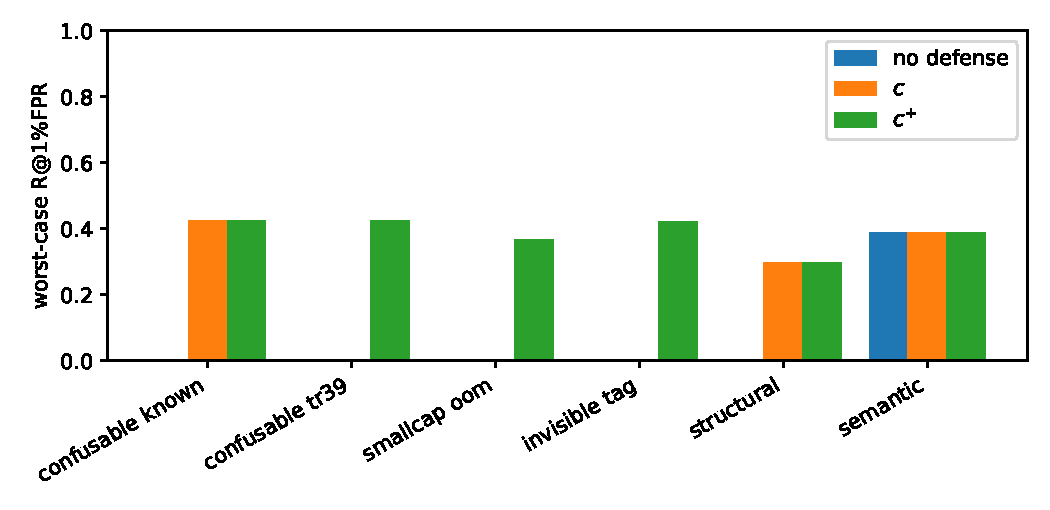
\includegraphics[width=\linewidth]{figures/fig2_adaptive_heldout.pdf}
\caption{Defense-aware adaptive attacker, leave-one-family-out, on InjecGuard.
Worst-case Recall@1\%FPR for the held-out family under no defense, base
canonicalization $c$, and the hardened canonicalizer $c^{+}$. The optimizer
collapses the undefended detector on every obfuscation family; $c^{+}$ recovers the
out-of-table families ($c$ does not), while semantic paraphrase is a no-op for both.}
\label{fig:adaptive}
\end{figure}

\subsection{Detector-agnostic recovery}
\label{sec:res-recovery}
Applied as a black-box pre-processor, canonicalization restores operational recall
across detectors (Table~\ref{tab:recovery}). It lifts InjecGuard's homoglyph and
zero-width recall from $\approx 0.00$ to $0.42$ and CANOPI's leet and spacing recall
from $0.68$ and $0.51$ to $0.96$ and $0.98$; DeBERTa-v3's over-trigger under
obfuscation is normalized to its clean value. The primitive thus recovers recall for
the detectors that are vulnerable to obfuscation, confirming detector-agnosticism in
practice as well as in theory.

% tab:recovery is generated from results_COSE/recovery/recovery_matrix_agg.csv
% (real-detector 5-seed run) by code/emit_tables.py. Do not edit by hand.
% AUTO-GENERATED by code/emit_tables.py from results_COSE/NUMBERS.json -- do not edit by hand.
\begin{table}[t]\centering
\caption{Detector-agnostic recovery, $\mathrm{R@1\%FPR}$ attacked vs. +canonicalization (5-seed mean $\pm$ s.d.).}
\label{tab:recovery}
\small
\begin{tabular}{lll}
\toprule
Detector & Attack & Attacked $\to$ +canon \\
\midrule
CANOPI (joint) & homoglyph & 0.9615 $\to$ 0.962 \\
CANOPI (joint) & zero\_width & 0.9615 $\to$ 0.962 \\
CANOPI (joint) & leet & 0.6825 $\to$ 0.96 \\
CANOPI (joint) & spacing & 0.512 $\to$ 0.9755 \\
Regex baseline & homoglyph & 0.019 $\to$ 0.1325 \\
Regex baseline & zero\_width & 0.0135 $\to$ 0.1325 \\
Regex baseline & leet & 0.02 $\to$ 0.0445 \\
Regex baseline & spacing & 0.021 $\to$ 0.0465 \\
B1 TF--IDF{+}LinearSVM & homoglyph & 0.6125 $\to$ 0.99 \\
B1 TF--IDF{+}LinearSVM & zero\_width & 0.141 $\to$ 0.99 \\
B1 TF--IDF{+}LinearSVM & leet & 0.473 $\to$ 0.9835 \\
B1 TF--IDF{+}LinearSVM & spacing & 0.894 $\to$ 0.925 \\
B2 DeBERTa-v3 & homoglyph & 0.996 $\to$ 0.9125 \\
B2 DeBERTa-v3 & zero\_width & 1.0 $\to$ 0.9125 \\
B2 DeBERTa-v3 & leet & 1.0 $\to$ 0.9435 \\
B2 DeBERTa-v3 & spacing & 1.0 $\to$ 0.951 \\
B3 InjecGuard & homoglyph & 0.0025 $\to$ 0.425 \\
B3 InjecGuard & zero\_width & 0.0 $\to$ 0.425 \\
B3 InjecGuard & leet & 0.3885 $\to$ 0.361 \\
B3 InjecGuard & spacing & 0.005 $\to$ 0.33 \\
\bottomrule
\end{tabular}
\end{table}


\subsection{The learned objective, in-domain and cross-lingual}
\label{sec:res-learned}
We report this result in full because it is partly negative. In-domain, on the
saturated xTRam1 benchmark, the joint objective gives no advantage over its own
ablations (Table~\ref{tab:main}): CANOPI reaches $0.959 \pm 0.005$, statistically
tied with its embedding ($0.954$), invariance-only ($0.962$), and partial-AUC-only
($0.958$) ablations (Holm-corrected McNemar $p=1.0$ for all three), while a TF--IDF
baseline reaches $0.988$. The same McNemar tests confirm CANOPI significantly exceeds
DeBERTa-v3 ($p<0.001$, Holm-corrected) and InjecGuard ($p \ll 0.001$) but ties the
saturated lexical and embedding baselines. Cross-lingual, the value of
the learned objective is conditional on the encoder. On a \emph{monolingual} encoder
the no-invariance probe collapses (Arabic $0.00$, Spanish $0.00$, Hindi $0.00$,
Russian $0.00$) and the invariance objective lifts the recoverable languages
(es\_mt $0.52$, fr\_mt $0.61$, de\_mt $0.40$, zh\_mt $0.51$), while honestly failing
on scripts the encoder discards (Arabic $0.015$, Hindi $0.024$, Russian $0.007$);
Figure~\ref{fig:crosslingual} shows this bounded effect. On
a \emph{multilingual} encoder this advantage disappears: the no-invariance probe
already reaches Arabic $0.76$ and Spanish $0.95$, matching or exceeding the joint
model. In short, the learned invariance objective is a conditional mechanism, useful
only when the backbone is monolingual and offering no in-domain gain; it does not
provide a general substitute for a multilingual encoder.

% tab:main is generated from results_COSE/in_domain/main_results_agg.csv
% (5-seed run) by code/emit_tables.py. Do not edit by hand.
% AUTO-GENERATED by code/emit_tables.py from results_COSE/NUMBERS.json -- do not edit by hand.
\begin{table}[t]\centering
\caption{In-domain detection on xTRam1, $\mathrm{R@1\%FPR}$ (5-seed mean $\pm$ s.d.; external baselines are single-valued, so their s.d. is $0$). The benchmark is in-domain-saturated; the joint objective gives no advantage over its ablations, which is why our contribution is the certified primitive and its adaptive evaluation, not an in-domain accuracy gain.}
\label{tab:main}
\small
\begin{tabular}{lc}
\toprule
Detector & $\mathrm{R@1\%FPR}$ \\
\midrule
Regex baseline & 0.136 $\pm$ 0.000 \\
B1 TF--IDF{+}LinearSVM & 0.988 $\pm$ 0.000 \\
B2 DeBERTa-v3 & 0.924 $\pm$ 0.000 \\
B3 InjecGuard & 0.427 $\pm$ 0.000 \\
CANOPI (joint) & 0.959 $\pm$ 0.005 \\
B5 embedding & 0.954 $\pm$ 0.005 \\
B6 invariance-only & 0.962 $\pm$ 0.004 \\
B7 partial-AUC-only & 0.958 $\pm$ 0.007 \\
\bottomrule
\end{tabular}
\end{table}


\begin{figure}[t]
\centering
\includegraphics[width=\linewidth]{figures/fig3_crosslingual_mono.pdf}
\caption{Cross-lingual recall at a frozen $1\%$ FPR threshold on a \emph{monolingual}
encoder. The no-invariance probe (B5) collapses, and the learned invariance objective
(CANOPI) recovers the languages the encoder retains signal for but cannot manufacture
signal for scripts it discards (Arabic, Hindi, Russian). On a multilingual encoder
this advantage disappears (B5 reaches Arabic $0.76$, Spanish $0.95$), so the effect is
conditional on a monolingual backbone.}
\label{fig:crosslingual}
\end{figure}

\subsection{Calibration, over-defense, and transfer}
The reference detector is well calibrated (ECE $0.065$, Brier $0.018$ after the
corrected estimator). Ranking transfers across corpora (deepset AUROC $0.83$) but the
in-domain threshold does not (recall at the fixed threshold $0.18$), and jailbreak
transfer recall is low ($0.22$), consistent with the scope taxonomy that places
semantic jailbreaks outside the method. We report one limitation prominently: at the
$1\%$ operating point the reference detector over-defends on the NotInject
hard-negative set (over-defense FPR $0.29$), comparable to the embedding baseline
($0.27$) and far worse than the over-defense-tuned InjecGuard ($0.018$;
Figure~\ref{fig:overdefense}). The
in-domain threshold does not transfer to adversarial-benign text; canonicalization
neither causes nor worsens this (it is FPR-neutral), but a deployment must
recalibrate the operating threshold on a target-benign slice.

\begin{figure}[t]
\centering
\includegraphics[width=0.78\linewidth]{figures/fig4_overdefense.pdf}
\caption{Over-defense at the $1\%$ operating point on the NotInject hard-negative
benchmark (lower is better). The reference detector over-defends comparably to the
other general detectors and far more than the over-defense-tuned InjecGuard; this is
an orthogonal limitation that input canonicalization does not address.}
\label{fig:overdefense}
\end{figure}

% ======================================================================
\section{Discussion}
\label{sec:discussion}
The results separate cleanly into a provable core and a conditional learned layer.
The certificate, its false-positive safety, and its survival under adaptive attack
(Sections~\ref{sec:res-cert}--\ref{sec:res-recovery}) are the contribution: they
hold by construction and in measurement, they
are detector-agnostic, and they answer the field's central complaint that defenses
fail once the attacker adapts, for the orthographic class at least. Positioned
against prior certified work, the guarantee is stronger on the obfuscation axis than
bounded-token erase-and-check~\cite{kumar2023} and is deterministic rather than
probabilistic like randomized smoothing~\cite{robey2023}; the trade is that it
certifies the orthographic/encoding class specifically rather than an arbitrary
perturbation ball.

The learned layer is reported honestly as conditional and, in-domain, redundant. We
view this as a feature of the framing rather than a weakness of the paper: because
the contribution is the certified primitive, it does not depend on the learned head
winning a benchmark. Two practical implications follow. First, where an operator
already runs a multilingual encoder, the canonicalization front end is sufficient and
the learned invariance objective can be omitted. Second, the over-defense behavior at
strict thresholds is an orthogonal problem that input normalization does not solve
and that deployments must address through target-specific recalibration.

\subsection{Limitations}
Our certificate covers information-preserving orthographic and encoding obfuscation,
not semantic paraphrase, persona or optimization-based jailbreaks, or multi-turn
attacks; these are out of scope by construction and we do not claim otherwise. The
cross-lingual study uses modest curated sets for Arabic and Spanish and a small
romanized-Arabic set; the monolingual-encoder substitution effect, while clear in
direction, is bounded in magnitude and fails on scripts the encoder discards. The
over-defense rate at $1\%$ FPR is a real usability cost for the reference detector.
Finally, the certified closure depends on the loaded UTS\#39 table; a novel
look-alike outside the standard would require a table update, which is why we pair
the certificate with the adaptive, hardened evaluation rather than relying on it
alone.

% ======================================================================
\section{Conclusion}
\label{sec:conclusion}
We showed that prompt-injection detectors can canonicalize before they classify, and
that a deterministic canonicalizer admits a decision-invariance certificate: attack
success over the entire Unicode confusable, invisible-character, and depth-bounded
encoding closure of an input is exactly zero, for any detector, with no retraining.
We made the certificate operational against the full Unicode standard while proving
and measuring that it does not cost false positives on genuine non-Latin text, and
we validated it under a defense-aware optimizer on held-out attack families, where a
hardened canonicalizer recovers detectors that base canonicalization cannot. We
additionally reported, in full, that a learned cross-lingual invariance objective is
conditional on a monolingual encoder and redundant on a multilingual one. The
certified primitive is the contribution, and it is released for reuse. Future work
should extend certified treatment toward the semantic frontier, for example by
pairing input-space canonicalization with representation-space defenses that target
meaning-preserving attacks.

% ======================================================================
\section*{CRediT authorship contribution statement}
\textbf{Shaikhah Alkhadhr:} Conceptualization, Methodology, Software, Formal
analysis, Writing -- original draft, Supervision. \textbf{Heba Alturki:} Software,
Validation, Data curation, Writing -- review \& editing. \textbf{Aseel Alghemlas:}
Investigation, Validation, Writing -- review \& editing.

\section*{Declaration of competing interest}
The authors declare that they have no known competing financial interests or
personal relationships that could have appeared to influence the work reported in
this paper.

\section*{Data availability}
The canonicalization package, the certificate checker, the defense-aware attacker,
and a one-run reproducibility notebook are released publicly; all benchmarks used are
publicly available datasets cited in the text.

\section*{Funding}
This research did not receive any specific grant from funding agencies in the
public, commercial, or not-for-profit sectors.

\section*{Declaration of Generative AI and AI-assisted technologies in the writing process}
During the preparation of this work the authors used a generative AI assistant in
order to support drafting, editing, and code scaffolding. After using this tool the
authors reviewed and edited the content as needed and take full responsibility for
the content of the publication.

% ======================================================================
\begin{thebibliography}{99}

\bibitem{greshake2023} K. Greshake, S. Abdelnabi, S. Mishra, C. Endres, T. Holz,
M. Fritz, Not what you've signed up for: Compromising real-world LLM-integrated
applications with indirect prompt injection, in: Proc. ACM Workshop on Artificial
Intelligence and Security (AISec), 2023.

\bibitem{liu2024usenix} Y. Liu, et al., Formalizing and benchmarking prompt
injection attacks and defenses, in: USENIX Security Symposium, 2024.

\bibitem{owasp2025} OWASP, LLM01:2025 Prompt Injection, OWASP Top 10 for LLM
Applications, 2025.

\bibitem{boucher2022} N. Boucher, I. Shumailov, R. Anderson, N. Papernot, Bad
characters: Imperceptible NLP attacks, in: IEEE Symposium on Security and Privacy,
2022.

\bibitem{li2025injecguard} H. Li, et al., InjecGuard: Benchmarking and mitigating
over-defense in prompt injection guardrail models, in: Annual Meeting of the
Association for Computational Linguistics (ACL), 2025.

\bibitem{promptshield2025} PromptShield: Deployable detection for prompt injection
attacks, in: ACM Conference on Data and Application Security and Privacy (CODASPY),
2025.

\bibitem{datasentinel2025} DataSentinel: A game-theoretic detection of prompt
injection attacks, in: IEEE Symposium on Security and Privacy, 2025.

\bibitem{inan2023llamaguard} H. Inan, et al., Llama Guard: LLM-based input-output
safeguard for human-AI conversations, arXiv:2312.06674, 2023.

\bibitem{wallace2024} E. Wallace, et al., The instruction hierarchy: Training LLMs to
prioritize privileged instructions, arXiv:2404.13208, 2024.

\bibitem{struq2025} S. Chen, et al., StruQ: Defending against prompt injection with
structured queries, in: USENIX Security Symposium, 2025.

\bibitem{secalign2025} S. Chen, et al., SecAlign: Defending against prompt injection
with preference optimization, in: ACM Conference on Computer and Communications
Security (CCS), 2025.

\bibitem{uts39} Unicode Consortium, Unicode Technical Standard \#39: Unicode Security
Mechanisms, 2023.

\bibitem{zhan2025} Q. Zhan, et al., Adaptive attacks break defenses against indirect
prompt injection attacks on LLM agents, in: Findings of NAACL, 2025.

\bibitem{attacker2025} The attacker moves second: Stronger adaptive attacks bypass
defenses against LLM jailbreaks and prompt injections, arXiv:2510.09023, 2025.

\bibitem{andriushchenko2024} M. Andriushchenko, F. Croce, N. Flammarion, Jailbreaking
leading safety-aligned LLMs with simple adaptive attacks, in: International
Conference on Learning Representations (ICLR), 2025.

\bibitem{kumar2023} A. Kumar, et al., Certifying LLM safety against adversarial
prompting, arXiv:2309.02705, 2023.

\bibitem{robey2023} A. Robey, E. Wong, H. Hassani, G. Pappas, SmoothLLM: Defending
LLMs against jailbreaking attacks, arXiv:2310.03684, 2023.

\bibitem{cohen2019} J. Cohen, E. Rosenfeld, J. Z. Kolter, Certified adversarial
robustness via randomized smoothing, in: International Conference on Machine Learning
(ICML), 2019.

\bibitem{camel2025} E. Debenedetti, et al., Defeating prompt injections by design
(CaMeL), arXiv:2503.18813, 2025.

\bibitem{melon2025} MELON: Provable defense against indirect prompt injection, in:
International Conference on Machine Learning (ICML), 2025.

\bibitem{liu2024cose} L. Liu, X. Kuang, L. Liu, L. Zhang, Defend against adversarial
attacks in malware detection through attack space management, Computers \& Security
(2024) 103841.

\bibitem{khosla2020} P. Khosla, et al., Supervised contrastive learning, in:
Advances in Neural Information Processing Systems (NeurIPS), 2020.

\bibitem{madry2018} A. Madry, et al., Towards deep learning models resistant to
adversarial attacks, in: International Conference on Learning Representations (ICLR),
2018.

\end{thebibliography}


\end{document}
